\begin{center}
{\huge\textbf{\ttitle}}\\
\end{center}
\section{Introduction and background}
\addcontentsline{toc}{section}{Introduction and background}
Sentiment analysis involves gathering individuals' viewpoints, feelings, assessments, judgments, perspectives, and emotional responses toward products and their distinct characteristics. This evaluation can occur across different tiers, such as analyzing entire documents, individual sentences, and specific attributes.
\\
Our objective is to assess the overall quality of a hospital from a patient's perspective, focusing on the quality of service provided to them. To achieve this, we rely on online reviews submitted by patients for a particular hospital. By analysing these reviews, we aim to extract fine-grained sentiment expressions.
\\
Unlike traditional methods that assess the overall sentiment of a sentence without considering specific aspects, we take a more nuanced approach. We classify the sentiment polarity of each aspect by carefully analysing the corresponding context, thus providing a more detailed and fine-grained solution.
\\
The primary goal of our project is to simultaneously identify aspect terms and their corresponding sentiment polarity pairs within a given patient review sentence. To accomplish this, we leverage user-generated data available on the \href{www.mouthshut.com}{mouthshut website} in the hospital category. This data serves as a valuable source for understanding patient experiences and evaluating the quality of care provided by different hospital environments.
\clearpage
\section{Literature survey}
\subsection{Web Scarping}
Web scraping is an automated method for extracting substantial amounts of data from websites. This process involves the utilization of web crawlers or bots to navigate through web pages, retrieve specific information, and store it for further analysis. Web scraping is essential for gathering data at scale, which is particularly valuable for research and analysis purposes.
\subsection{Text cleaning}
Text cleaning is a critical preliminary step in Natural Language Processing (NLP). This phase entails a series of operations such as tokenization, lowercasing, removal of special characters, stop words, and stemming or lemmatization. These operations help in cleaning and transforming unstructured text data into a more structured and analyzable format. Effective text pre-processing enhances the quality of NLP tasks, including sentiment analysis.
\subsection{Automated Data Annotation}
Automated data annotation is achieved through the utilization of advanced pre-trained language models and the application of transfer learning techniques. This approach allows data to be labeled or annotated intelligently without manual human intervention. By leveraging the capabilities of state-of-the-art models like BERT (Bidirectional Encoder Representations from Transformers), the process of assigning labels or sentiment scores to data becomes efficient and accurate.
\subsection{Model Training & Evaluation}
Model training involves formatting the annotated dataset for a specific machine learning model. The choice of format depends on the type of model being used. In this research project, we employ an instruction-based text generative model, which requires a particular input data structure. The model is trained using available pre-trained models as a base, which leverages the knowledge learned from extensive text corpora. The training process involves optimizing the model's parameters to fit the task of sentiment analysis. For evaluation, a dedicated test dataset is employed to assess the model's performance. This evaluation helps determine whether the trained model aligns with the predefined objectives, effectively capturing user sentiments in the context of the specific aspects analyzed.
\subsection{KeyBERT}
KeyBERT is a sophisticated aspect extraction technique that leverages BERT embeddings and cosine similarity. It identifies and extracts important aspects or phrases within a sentence. This technique assesses the weightage of words in the context of the entire document or sentence, allowing for the identification of critical terms that encapsulate the essence of the text.
\clearpage
\section{Problem definition and Objective}
This project encompasses several essential phases with the goal of extracting valuable insights from hospital online reviews. The primary objectives and steps are outlined below.
\\
In the initial phase, we implement automated web scraping techniques to systematically gather hospital online reviews from diverse customers. This process involves the systematic extraction of relevant data from open-source websites. The data collected during this phase serves as the fundamental building block for our subsequent analysis.
\\
Following data acquisition, we apply a range of Natural Language Processing (NLP) techniques to the collected data. These techniques encompass text pre-processing, aspect-level data annotation, model development, and model training. To ensure robust model performance, we allocate the annotated data into a 75/15/10 ratio for training, validation, and testing, respectively.
\\
To facilitate effective model training, we embark on the creation of custom training datasets. This phase is instrumental in enhancing the quality of our analysis. To achieve this, we leverage both 'english' and 'multilingual' & KeyBERT-based pre-trained model checkpoints for annotating the training data. The objective here is to construct high-quality annotated training data using automated annotation and save time, a crucial component of our analysis.
\\
In this step, we engage in model training and evaluation. Our objective is to train machine learning models and rigorously evaluate their performance. We use crucial metrics like Precision, Recall, and F1 Score for assessment. This assessment extends to both the training dataset and an unseen test dataset. Additionally, we employ visual aids to present the training and validation progress, including loss values.
\\
To gain deeper insights into our approach, we conduct a comparative analysis of the results obtained from three different annotation methods: 'english,' 'multilingual,' and KeyBERT-based annotation. This comparison is conducted on an unseen test sample, allowing us to discern the most effective approach for achieving our research objectives.
\clearpage
\section{Approach}
\subsection{Gathering and Preparing Data}
To source our data, I employed python based web scraping techniques on the \href{www.mouthshut.com}{mouthshut website}. The goal was to gather online reviews provided by customers for various hospitals. I systematically extracted unstructured data, which included customer reviews, summaries, and ratings. Subsequently, this data was meticulously organized and stored in Excel-based file. In total, I successfully extracted 56,080 reviews, summaries, and corresponding ratings from different hospitals. This comprehensive dataset forms the foundation for the analysis and allows me to delve into the fine-grained sentiment analysis of hospital service quality.
\subsection{Text Cleaning for Aspect Extraction}
In the process of preparing data for aspect extraction from online reviews, we executed a series of Natural Language Processing (NLP) text cleaning approach to ensure the cleanliness and reliability of the dataset. This phase comprised several distinct steps aimed at enhancing the quality of the text data:
\begin{enumerate}
    \item \textbf{Stripping HTML Tags:} The initial step involved the removal of HTML tags from the content, ensuring that our analysis relied solely on the textual data.
    
    \item \textbf{Removing Accented Characters:} Accented characters were systematically removed from the text, standardizing character representations to achieve consistency and facilitate analysis.
    
    \item \textbf{Expanding Contractions:} To enhance text clarity, we expanded contractions. For instance, 'you've' was transformed to 'you have,' preserving the intended meaning.
    
    \item \textbf{Removing Special Characters and Digits:} Special characters and digits were eliminated to isolate the textual content, improving readability and relevance for analysis.
    
    \item \textbf{Handling Repeated Characters:} Addressing the presence of repeated characters was crucial for accurate sentiment analysis. For example, 'happppppy' was normalized to 'happy' for consistency.
    
    \item \textbf{Eliminating Stop Words:} Common stop words, such as 'and,' were removed to reduce noise and emphasize content with more substantial meaning.
    
    \item \textbf{Splitting Words:} In cases where combined words lacked spaces, we separated them into their correct forms. For instance, 'doctoris' was split into 'doctor is,' enhancing the text's interpretability.
\end{enumerate}
\\
The implementation of these text pre-processing techniques played a pivotal role in the thorough cleaning and refinement of online reviews, ensuring that subsequent aspect extraction would be based on accurate and structured data. This meticulous preparation is integral to achieving precise results in our analysis.
\subsection{Data Annotation for Aspect-Based Sentiment Analysis}
In this phase, we meticulously prepared the data through automated aspect-sentiment based annotation, employing state-of-the-art open-source pre-trained models. Our objective was to address the challenges posed by limited data and reduce human involvement through automatic annotation methods.
\\
To facilitate this process, we utilized the PyABSA library's 2.2.0 version, specifically leveraging the 'make\_ABSA\_dataset' function. This method allowed us to automatically annotate the data and enrich it with aspect-based sentiment labels.
\\
We incorporated both 'english' and 'multilingual' versions of the E2EABSA. The 'english' checkpoint model was trained on the "SemEval" dataset, while the 'multilingual' checkpoint model was trained on a combination of "SemEval + Synthetic + Chinese\_Zhang datasets." Both models utilized the "FAST-LCF-ATEPC" architecture based on BERT, ensuring robust and accurate annotations.
\\
Additionally, we applied KeyBERT, utilizing two different models. The first model, sourced from \href{https://huggingface.co/sentence-transformers/all-MiniLM-L6-v2}{allMiniLML6v2} pre-trained transformer based embedding model. This model has been trained on an extensive dataset of 1 billion sentence pairs, enabling it to map sentences and paragraphs into a dense 384-dimensional vector space. The second model, from \href{https://huggingface.co/yangheng/deberta-v3-base-absa-v1.1}{yangheng-deberta-v3-base-absa-v1.1}, is a pre-trained sentiment model trained on over 30,000 ABSA samples, allowing it to effectively extract both aspects and sentiments from the text.
\\
The application of these advanced models and automatic annotation methods ensures the precision and depth of the aspect-based sentiment analysis in our research, contributing to the reliability and richness of our findings.
\subsection{Model Development for Aspect-Sentiment Analysis}
In the model development phase, we employed a powerful open-source text generative base model, namely, the \href{https://huggingface.co/allenai/tkinstruct-base-def-pos}{allenai-tkinstruct-base-def-pos}, This model was based on an encoder-decoder transformer architecture, specializes in solving sequence-to-sequence (seq2seq) NLP tasks. It was trained using the annotated data we prepared earlier, enabling it to generate aspects and their corresponding sentiments as a single string output.
\\
This model's capabilities in sequence generation and sentiment aspect pairing are instrumental in our research, facilitating the extraction of nuanced aspect-based sentiment analysis results. The application of this model forms a pivotal component of our project's methodology, allowing us to derive valuable insights from the data.
\\
By utilizing this advanced model, we ensure the robustness and precision of our aspect-sentiment analysis, contributing to the depth and quality of our research findings.
\subsection{Model Training}
In this phase, we executed the training of our model, leveraging three distinct annotated datasets, namely 'english,' 'multilingual,' and 'KeyBERT.' To ensure the robustness of our model, we thoughtfully divided each dataset into specific train, validation, and test datasets, following a ratio of 75/15/10. For the model input, we formatted the training dataset with two crucial columns:
\begin{itemize}
    \item \textbf{Rawtext Column:} This column contained the cleaned review text, ensuring that our model was trained on high-quality and sanitized textual data.
    \item \textbf{AspectTerms Column:} This column included aspect terms in the format \[{’term’: <>, ’polarity’: <>}, {’term’: <>, ’polarity’: <>}, ...\]. These aspect terms, along with their associated polarities, played a pivotal role in training pre-trained model specifically for extracting aspects and its sentiments.
\end{itemize}
We utilized an instruct based text generative-based model to for fine-tuned training on this meticulously prepared dataset. This training process ensures that our model can effectively capture the nuances in user sentiment as related to specific aspects, resulting in a more detailed and precise analysis of the data. The comprehensive utilization of these datasets and the fine-tuned model training enhance the accuracy and depth of our aspect-based sentiment analysis, enabling us to derive valuable insights from the data with high precision.
\subsection{Model evaluation}
This section illustrates the evaluation of the final fine aspects and sentiments text geneartive trained model across three distinct datasets: English, Multilingual, and KeyBERT. We have conducted a comprehensive assessment by calculating precision, recall, and F1 validation metrics on the training, validation, and test data sets.
\\
\textbf{Performance Metrics}
\begin{itemize}
\item \textbf{Precision}: This metric reflects an accurate model's positive predictions.
\item \textbf{Recall}: Recall metric reflects an ability for model to interpret relevant instances.
\item \textbf{F1 Score}: It offers a well-rounded evaluation of the model's performance.
\end{itemize}
\subsection{Results on Training, Validation, and Test Data}
The fine tuned trained models of english, multilingual and keybert annotation startegies were accessed on Training, Validation, and Test datasets using recall, precision, and F1 score.
\end{itemize}
\subsection{Comparative Assessment}
In addition to the evaluation on the final trained model, we have conducted a comparative analysis by testing three different trained models on two sample test datasets. This approach allows us to gauge the performance differences between models and provides valuable insights into their capabilities.
\clearpage
\section{Theoretical/Numerical/Experimental findings}
The experiments were conducted on a GPU (Graphics Processing Unit) P100 GPU Memory - 15.9 GB, RAM - 29 GB computing platform as part of our methodology to attain the project's defined objectives.
\subsection{Text cleaning}
\begin{itemize}
\item \textbf{patient raw review}: "The hospital maheer is a good hospital and the doctors of a hospital are good to treat a patient and the hospital is a good and cleaned one I think all patients should get treatment in this hospital"
\item \textbf{patient cleaned review}: "the hospital me here is a good hospital and the doctors of a hospital are good to treat a patient and the hospital is a good and cleaned one I think all patients should get treatment in this hospital"
\end{itemize}
\subsection{Data counts}
\begin{itemize}
\item \textbf{Number of Train cleaned review data}: 16956
\item \textbf{Number of Valid cleaned review data}: 3239
\item \textbf{Number of Test cleaned review data}: 1000
\end{itemize}
\subsection{Annotated Data label count trends}
\begin{table}[h!]
\centering
 \begin{tabular}{c c c c c} 
 \hline
 SN & Annotation Method & Train & Valid & Test \\ [0.5ex] 
 \hline
 1 & English & 26877 & 5214 & 1629 \\ 
 2 & Multilingual & 31175 & 6069 & 1865 \\
 3 & KeyBERT & 79595 & 15218 & 4684 \\ [1ex] 
 \hline
 \end{tabular}
 \caption{\label{tab:mytab1} Aspects/Sentiments Label counts.}
\end{table}
\subsection{Model Training Hyperparameters}
\begin{table}[h!]
\centering
 \begin{tabular}{c c c c c} 
 \hline
 SN & Annotation Method & Batch Size & Epoch & Learning rate \\ [0.5ex] 
 \hline
 1 & English & 8 & 4 & 5e-5 \\ 
 2 & Multilingual & 8 & 4 & 5e-5 \\
 3 & KeyBERT & 4 & 8 & 5e-5 \\ [1ex] 
 \hline
 \end{tabular}
 \caption{\label{tab:mytab2} Hyperparameters.}
\end{table}
\subsection{Model Training and Predictions results}
\begin{figure}[h]
    \centering
    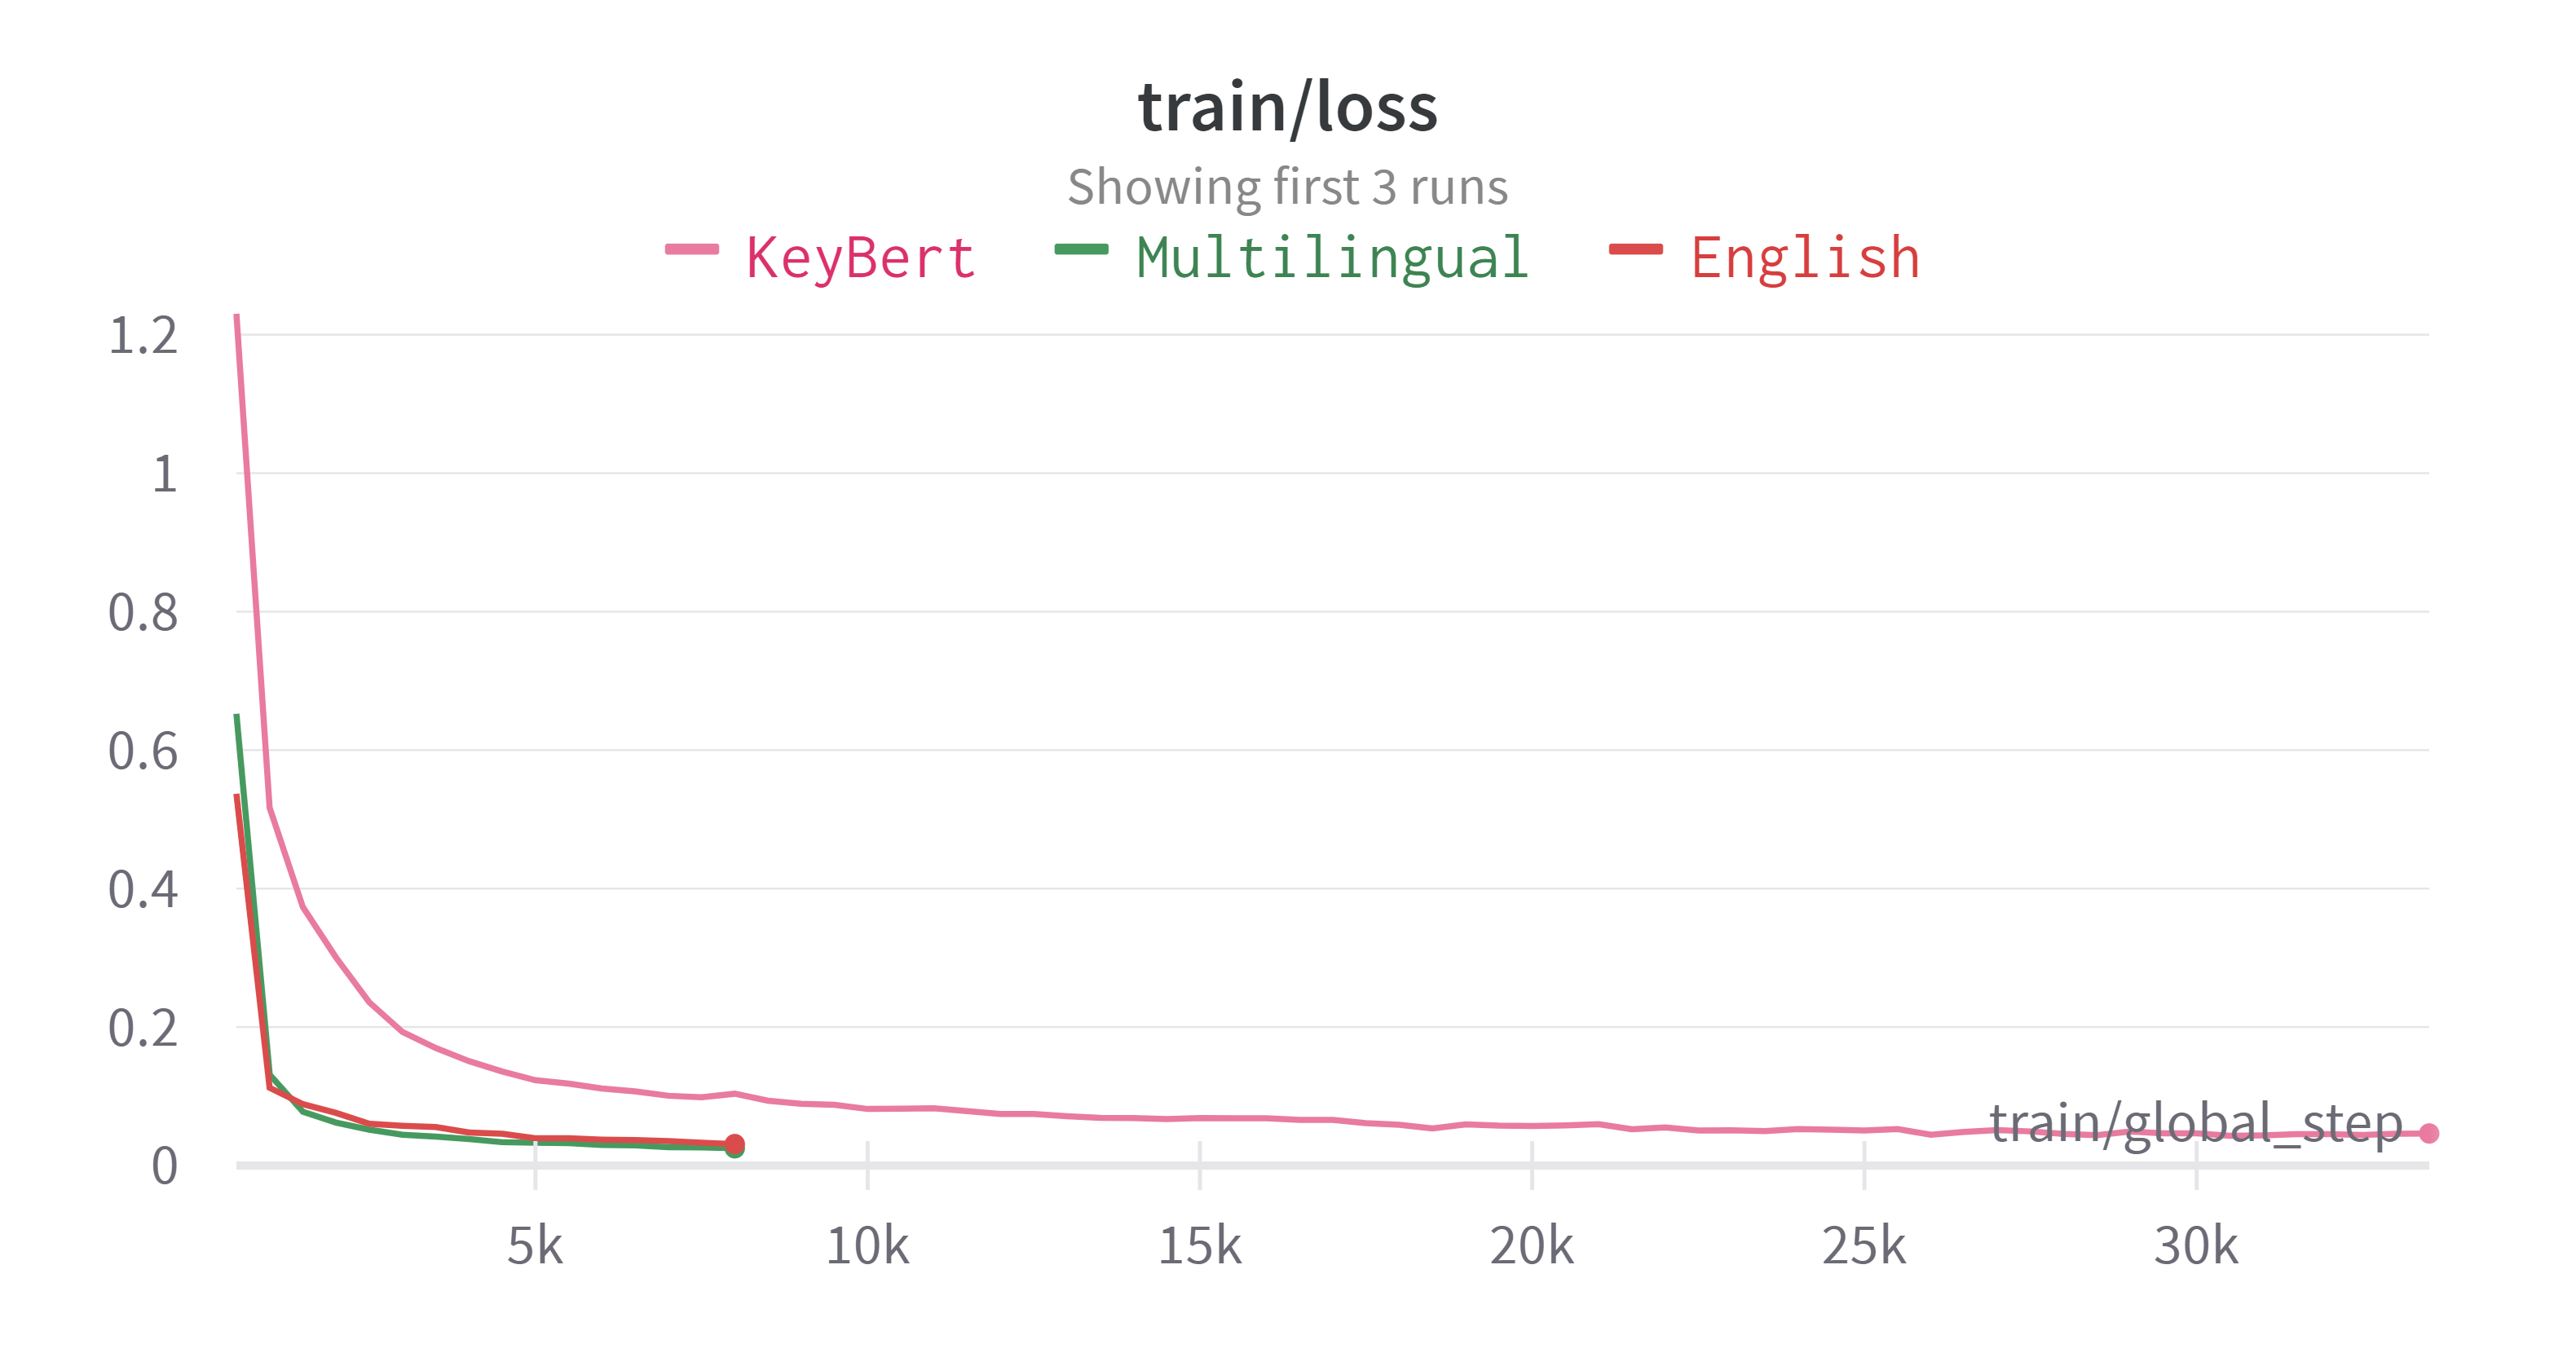
\includegraphics[width=0.80\textwidth,height=0.35\textwidth]{Figures/TrainLoss.png}
    \caption{\label{fig:myfig1}Train Loss Graph}
\end{figure}
\begin{figure}[h]
    \centering
    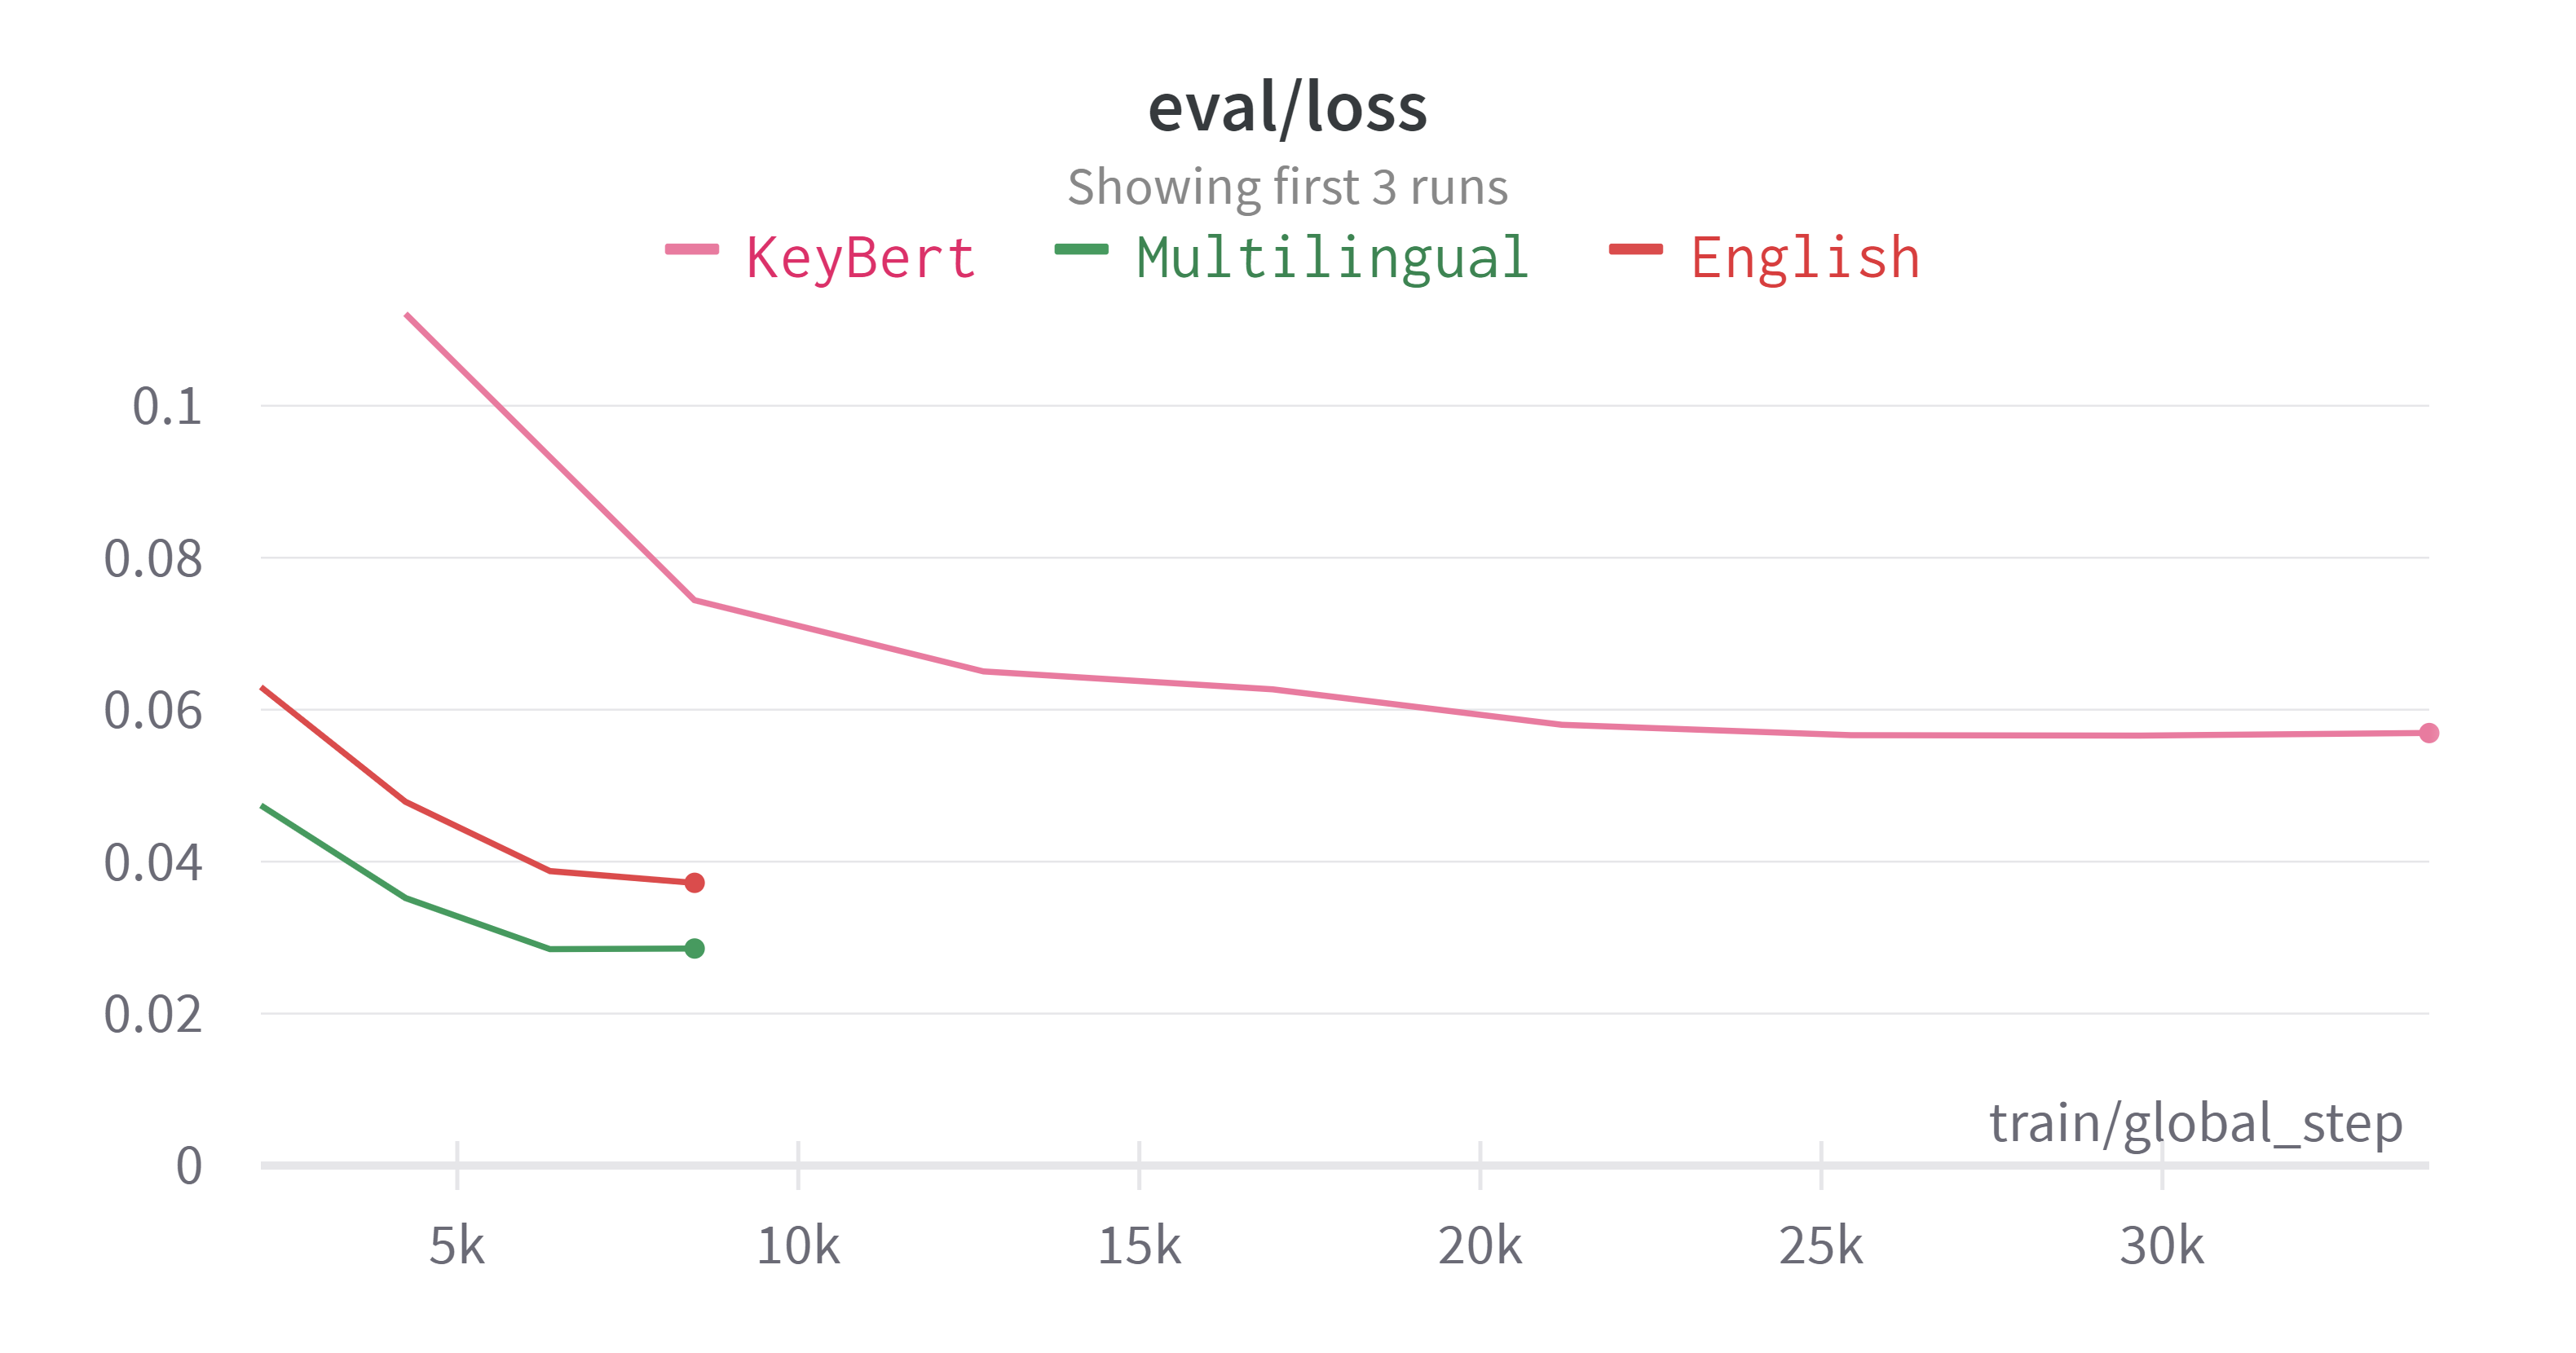
\includegraphics[width=0.80\textwidth,height=0.35\textwidth]{Figures/ValidLoss.png}
    \caption{\label{fig:myfig2}Valid Loss Graph}
\end{figure}

\begin{table}[h!]
\centering
 \begin{tabular}{c c c c c c c c} 
 \hline
 SN & Annotation Method & Dataset & Precision & Recall & F1 & Batch Size & Max Len \\ [0.5ex] 
 \hline
 1 & English & Train & 0.951679124 & 0.958439355 & 0.955047277 & 16 & 128 \\ 
 2 & English & Valid & 0.953347969 & 0.954046137 & 0.953696925 & 16 & 128 \\ 
 3 & English & Test & 0.954944412 & 0.953828171 & 0.954385965 & 16 & 128 \\ 
 4 & Multilingual & Train & 0.96826887 & 0.969209084 & 0.968738749 & 16 & 128 \\
 5 & Multilingual & Valid & 0.965 & 0.962051777 & 0.963523633 & 16 & 128 \\
 6 & Multilingual & Test & 0.967050209 & 0.968569932 & 0.967809474 & 16 & 128 \\
 7 & KeyBERT & Train & 0.955222755 & 0.955210754 & 0.955216755 & 16 & 512 \\
 8 & KeyBERT & Valid & 0.930091984 & 0.930153098 & 0.93012254 & 16 & 512 \\
 9 & KeyBERT & Test & 0.932963279 & 0.932963279 & 0.932963279 & 16 & 512 \\ [1ex] 
 \hline
 \end{tabular}
 \caption{\label{tab:mytab3} Prediction Results.}
\end{table}
\\
\begin{table}[h!]
\centering
 \begin{tabular}{c} 
 \hline
 This hospital has doctors who gave me the best consultation even though it was not \\ what other doctors would say. I was completely fine now because i followed thier advice. \\ [0.5ex] 
 \hline
 English - doctors:Positive, consultation:Positive  \\ 
 Multilingual - doctors:Positive, consultation:Positive  \\
 KeyBERT - hospital:Positive, consultation:Positive, doctors:Positive, best:Positive, probably:Positive  \\ [1ex] 
 \hline
 \end{tabular}
 \caption{\label{tab:mytab4} Unseen Test samples data Predictions.}
\end{table}
\clearpage
\section{Web Application to Enhance User Experience}
\subsection{Hosted WebApp Link and Code Files}
\begin{itemize}
\item \textbf{Web Application Link}: 
\href{https://huggingface.co/spaces/amir22010/HospitalReviewAspectSentimentExtraction}{amir22010/HospitalReviewAspectSentimentExtraction}
\item \textbf{Web Application Code Files}: 
\href{https://huggingface.co/spaces/amir22010/HospitalReviewAspectSentimentExtraction/tree/main}{amir22010/HospitalReviewAspectSentimentExtraction/tree/main}
\end{itemize}
\subsection{Deployed Custom Trained Models on Hugging Face Models}
\begin{itemize}
\item \textbf{English}: 
\href{https://huggingface.co/amir22010/PyABSA_Hospital_English_allenai_tk-instruct-base-def-pos_FinedTuned_Model}{amir22010/PyABSA\_Hospital\_English\_allenai\_tk-instruct-base-def-pos}
\item \textbf{Multilingual}: 
\href{https://huggingface.co/amir22010/PyABSA_Hospital_Multilingual_allenai_tk-instruct-base-def-pos_FinedTuned_Model}{amir22010/PyABSA\_Hospital\_Multilingual\_allenai\_tk-instruct-base-def-pos}
\item \textbf{KeyBERT}: 
\href{https://huggingface.co/amir22010/KeyBert_ABSA_Hospital_Multilingual_allenai_tk-instruct-base-def-pos_FinedTuned_Model}{amir22010/KeyBert\_ABSA\_Hospital\_Multilingual\_allenai\_tk-instruct-base-def-pos}
\end{itemize}
\subsection{Web Application}
\begin{figure}
    \centering
    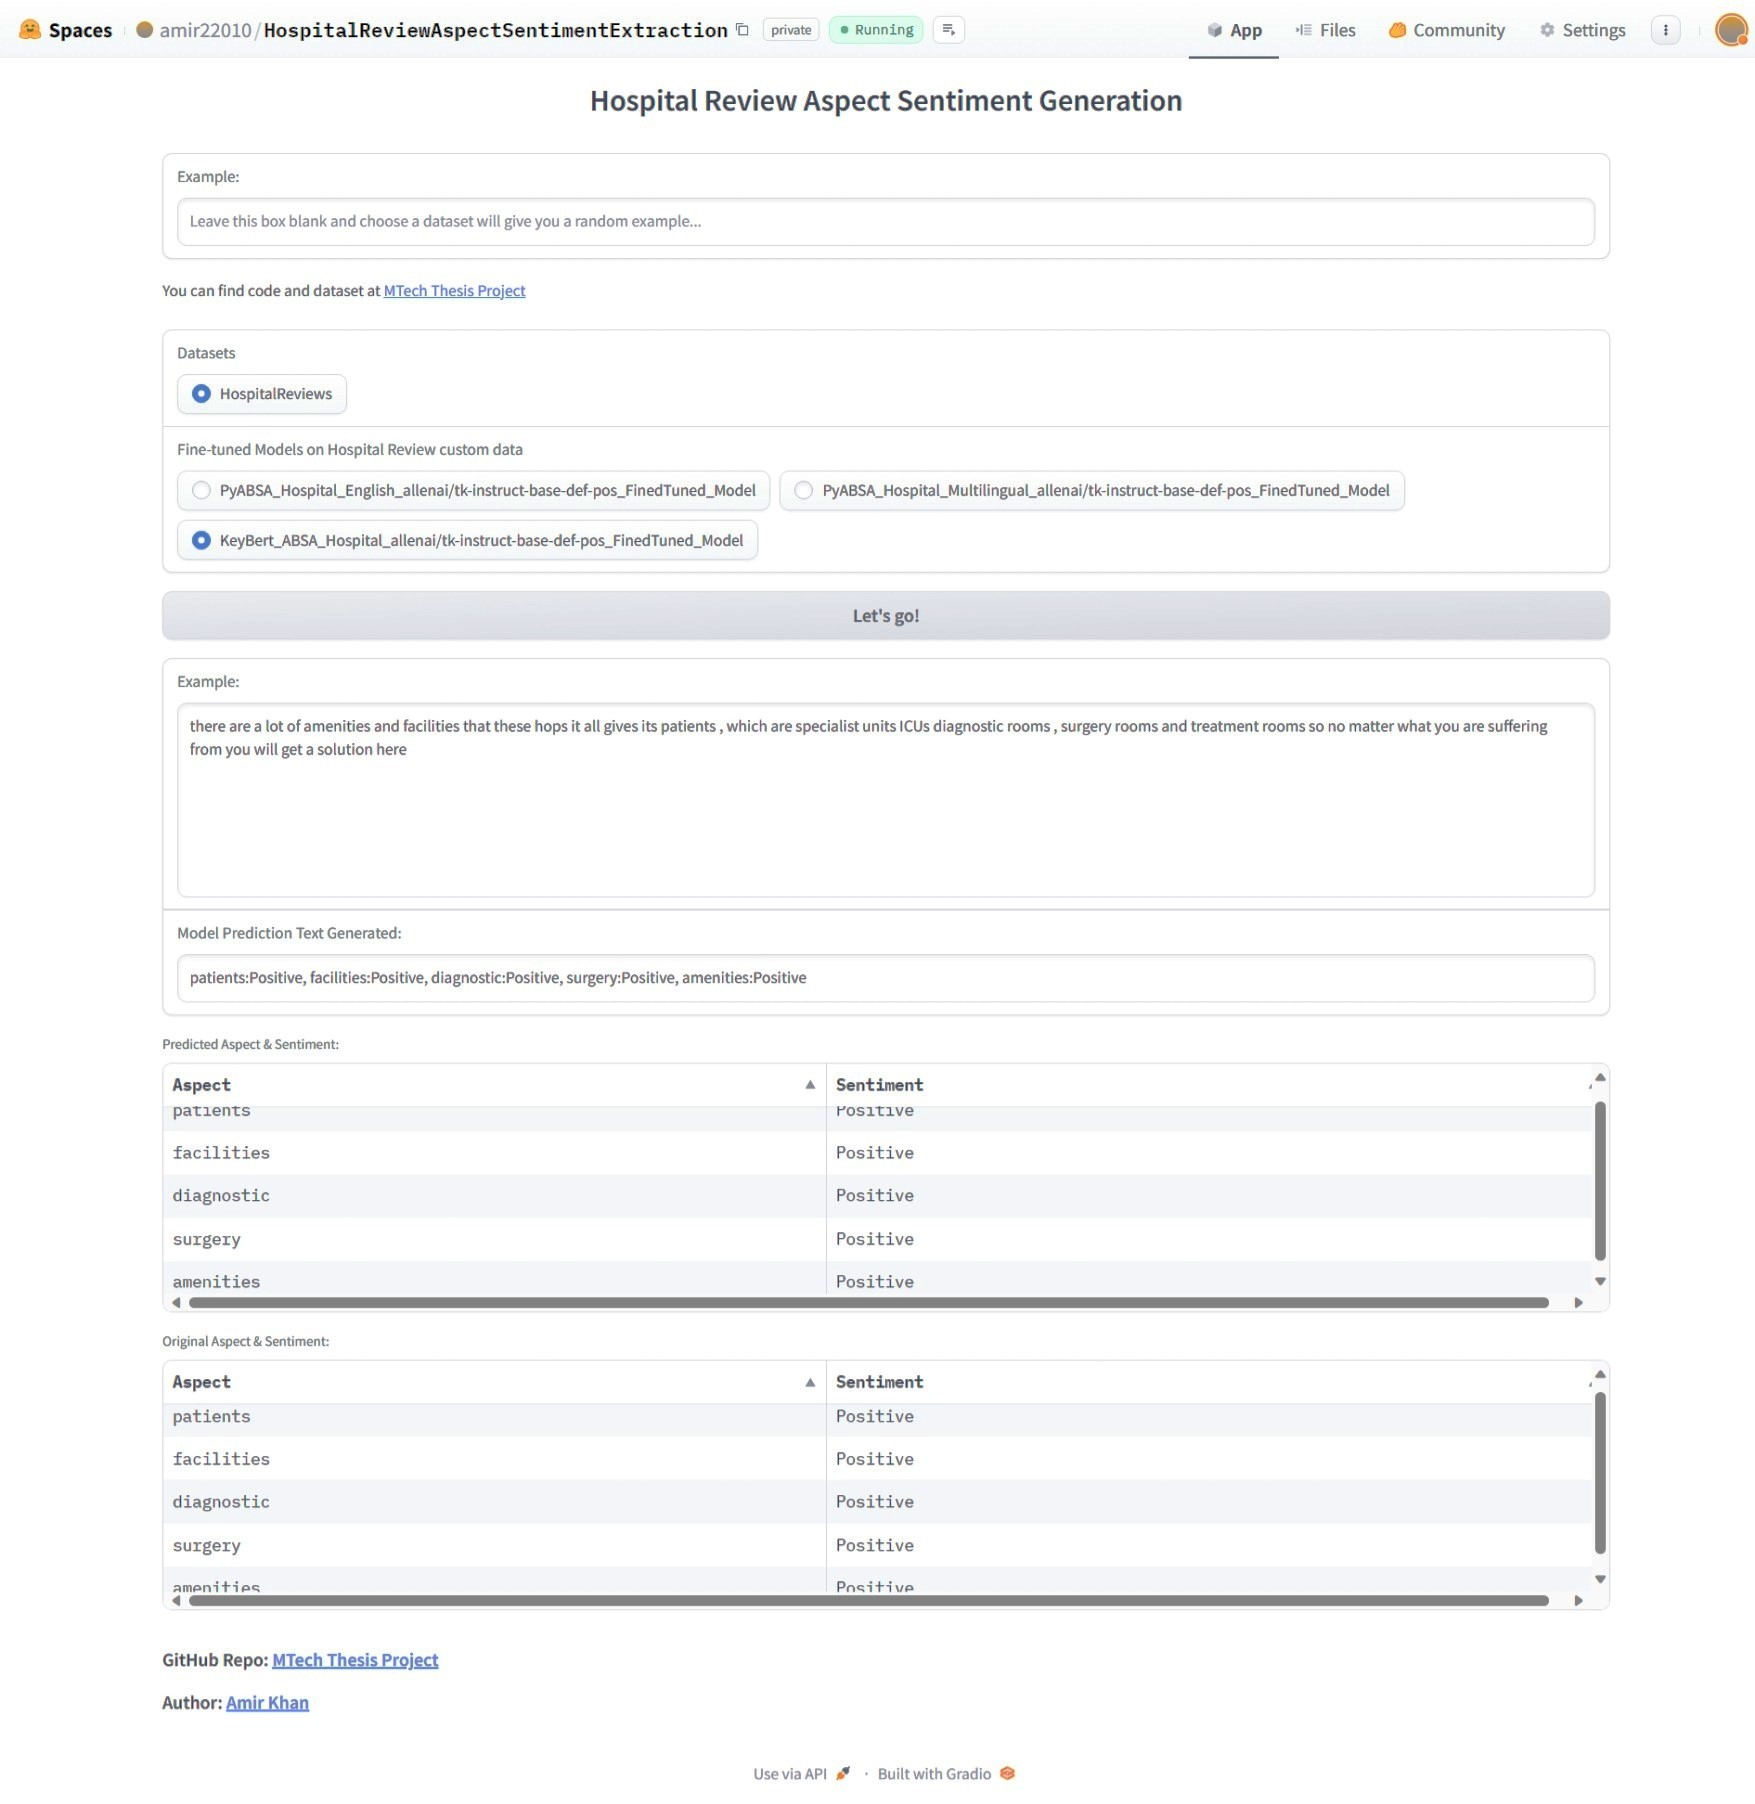
\includegraphics[width=1.2\linewidth]{Figures/WebApp.jpeg}
    \caption{Hosted Web Application on Hugging Face space platform}
    \label{fig:myfig3}
  \end{figure}
\clearpage
\section{Summary and Future Projected Work}
In this project, I have implemented automatic annotation using PyABSA pre-trained models [English, Multilingual] checkpoints and KeyBERT+\href{https://huggingface.co/allenai/tk-instruct-base-def-pos}{allenai-tk-instruct-base-def-pos} open-source pre-trained ABSA model and compared the total number of label counts in terms of aspects and sentiments extraction.
\\
I have also compared the training and validation accuracy for three different annotation startegy trained on instruct based text generative model.
\\
I have also shown the results by comparing three different custom fine-tuned text geneartive model trained on [English, Multilingual, KeyBERT] aspects extraction strategy on one sample in the report.
\\
By implemented this work, I have improved the capabilities of extracting aspects and sentiments by introducing only one AI model, in order to save time and computing resource.
\\
I will further improve the aspects and sentences extraction and doing human level improved automatic annotation by introducing KeyBERT and open-source Large Language model \href{https://huggingface.co/mistralai/Mistral-7B-Instruct-v0.1}{mistralai-Mistral-7B-Instruct-v0.1} together.
\subsection{Text Cleaning for Improved Aspect Extraction}
To enhance aspect extraction, we will further refine our text cleaning method.
\subsection{Incorporating Manual Annotation and Performance Evaluation}
We will integrate the manual annotation into our workflow and subsequently assessing fine tuned model performance in comparison to automatic annotation.
\subsection{Enhancing Testing Accuracy of KeyBERT-Based Annotation}
To improve the testing accuracy of our KeyBERT-based annotation method, we will extend the training process by increasing the number of epochs and closely monitoring the results.
\subsection{Compare KeyLLM (KeyBERT+LLM) and KeyBERT+FinedTunedInstructABSA model implemented in this project work}
To improve the testing accuracy of the aspects extraction, I will compare our Fine tuned KeyBERT-based Instruct text generative model on hospital reviews dataset with the KeyBERT+\href{https://huggingface.co/mistralai/Mistral-7B-Instruct-v0.1}{LLM} (generative ai based model), and look out more better approach by Incorporating the cutting edge improved generative ai model to extract better aspects and further extend the research work.
\subsection{Extracting Opinions}
To move forward with this project, i will also introduce \textbf{Opinions} extraction to further improve the overall understanding of the reviews.
\clearpage
\section*{Publications  (if any)}
\addcontentsline{toc}{section}{Publications  (if any)}
\begin{itemize}
    \item Amit Singh (Indian Institute of Technology Jodhpur, India), Mamata Jenamani (Indian Institute of Technology, Kharagpur, India), Jitesh Thakkar (National Rail and Transportation Institute, Vadodara, India), and Yogesh K. Dwivedi (Swansea University, UK), “A Text Analytics Framework for Performance Assessment and Weakness Detection from Online Reviews,” Journal of Global Information Management Volume 30 • Issue 8.
    \item Amit Singh, Mamata Jenamani and Jitesh Thakkar Department of Industrial and Systems Engineering, Indian Institute of Technology Kharagpur, Kharagpur, India, “Do online consumer reviews help to evaluate the performance of automobile manufacturers?,” Journal of Enterprise Information Management Issue(s) available: 114 – From Volume: 17 Issue: 1, to Volume: 36 Issue: 3
    \item Kevin Scaria, Himanshu Gupta, Siddharth Goyal, Saurabh Arjun Sawant, Swaroop Mishra, Chitta Baral, Arizona State University “InstructABSA: Instruction Learning for Aspect Based Sentiment Analysis,” 16	eb 2023 https://arxiv.org/abs/2302.08624
    \item Heng Yang, Chen Zhang, Ke Li, Department of Computer Science, University of Exeter, EX4 4QF, Exeter, UK, School of Computer Science, Beijing Institute of Technology, Beijing, China “A Modularized Framework for Reproducible Aspect-based Sentiment Analysis”, 23 Feb 2023 CoRR abs/2208.01368  https://doi.org/10.48550/arXiv.2208.01368
\end{itemize}
\clearpage
\section*{Appendix (if any)}
\addcontentsline{toc}{section}{Appendix (if any)}
\begin{itemize}
    \item \url{https://github.com/MaartenGr/KeyBERT}
    \item \url{https://pyabsa.readthedocs.io/en/v2/7_datasets/customized_datasets.html}
    \item \url{https://github.com/kevinscaria/InstructABSA}
    \item \url{https://huggingface.co/models}
    \item \url{https://huggingface.co/docs/transformers/v4.30.0/main_classes/text_generation}
    \item \url{https://www.kaggle.com/}
\end{itemize}